\begin{Antwoord}{1.1b}
            Je moet een uur terug tellen van de tijd die het nu is.
        
\end{Antwoord}
\begin{Antwoord}{1.3}
         Bissectrice
    
\end{Antwoord}
\begin{Antwoord}{1.5}
        Om 12 uur, ofwel het middaguur, staat de Zon recht in het zuiden. \textcolor{red}{aanvullen}
    
\end{Antwoord}
\begin{Antwoord}{1.6}
        Dicht bij de evenaar zijn de schaduwen korter en lijkt de zon altijd recht boven je te staan (en door de tilt van de aardas - $23.5^{\circ}$ werkt deze methode niet tussen de Kreeftskeerkring en de Steenbokskeerkring).
    
\end{Antwoord}
\begin{Antwoord}{1.7}
        Bepaal de kleinste hoek tussen de kleine wijzer en de 11. De bissectrice van deze hoek wijst nu recht naar het zuiden.
    
\end{Antwoord}
\begin{Antwoord}{1.8}
        Je hoeft geen rekening meer te houden met zomertijd, de zon staat lager dus je kan makkelijker de richting van de schaduwen bepalen.
    
\end{Antwoord}
\begin{Antwoord}{1.10}
        Richt de 12 van je horloge naar de zon, de bissectrice tussen de 12 en de kleine wijzer wijst nu naar het noorden.
    
\end{Antwoord}
\begin{Antwoord}{2.1a}
			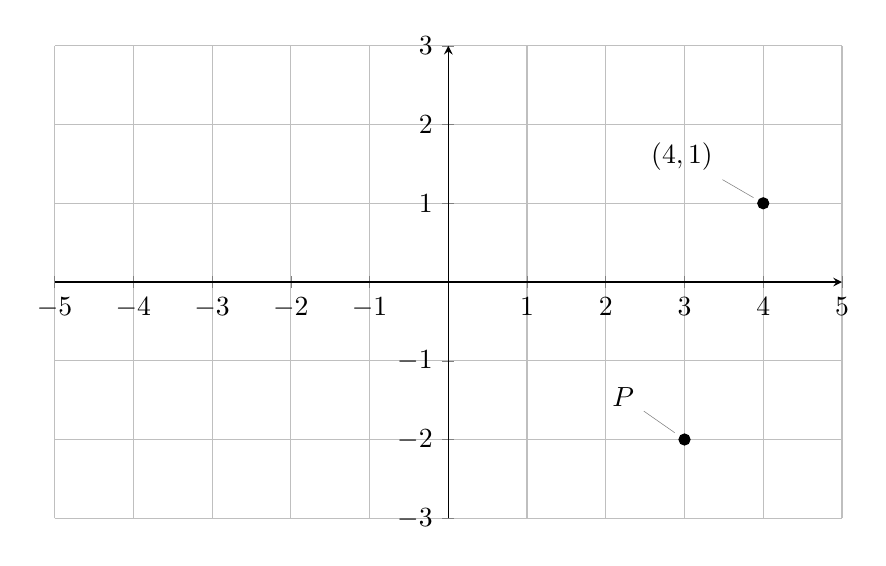
\begin{tikzpicture}
			    \begin{axis}[axis lines = middle, grid = both,
		                 xmin = -5, xmax = 5, ymin = -3, ymax = 3,
                		 x = 1cm, y = 1cm,
        		         xtick = {-5, -4, -3, -2, -1, 0, 1, 2, 3, 4,5},
		                 ytick = {-3, -2, -1, 0, 1, 2, 3}]
			        \addplot[mark=*] coordinates {(3,-2)} node[pin=150:{$P$}]{} ;
			        \addplot[mark=*] coordinates {(4,1)} node[pin=150:{$(4, 1)$}]{} ;
			    \end{axis}
			\end{tikzpicture}
		
\end{Antwoord}
\begin{Antwoord}{2.1b}
			$(3, -2)$
		
\end{Antwoord}
\begin{Antwoord}{2.2}
		Neem een cirkel, deze stelt de $360\degree$ aan lengtegraden op de evenaar voor. Roteer de cirkel nu om een as die door het midden van deze cirkel loopt. Bij het roteren vormt zich een boloppervlak. Merk op dat de cirkel slechts $180\degree$ geroteerd hoeft te worden om een volledige bol te maken, niet $360\degree$. Als de breedtegraden ook een bereik van $360\degree$ zouden hebben, dan zou ieder punt op Aarde twee sets co\"ordinaten hebben.
	
\end{Antwoord}
\begin{Antwoord}{2.3a}
			12800 km * $\pi$ = 40200 km
		
\end{Antwoord}
\begin{Antwoord}{2.3b}
			1/360 * 40200 km = 112 km
		
\end{Antwoord}
\begin{Antwoord}{2.3c}
			24500 km
		
\end{Antwoord}
\begin{Antwoord}{2.3d}
			$\frac{24500}{360} = 68$~km
		
\end{Antwoord}
\begin{Antwoord}{2.4}
		Ja.
	
\end{Antwoord}
\begin{Antwoord}{2.5a}
			Nee, de afstand tussen meridianen neemt af naarmate je verder van de evenaar komt en wordt 0 bij de polen.
		
\end{Antwoord}
\begin{Antwoord}{2.5b}
			Afstanden die gelijk zijn in de vlakke projectie zijn niet noodzakelijkerwijs gelijk op het boloppervlak. De projectie is dus niet afstand-behoudend.
		
\end{Antwoord}
\begin{Antwoord}{2.6a}
			Z (zuid)
		
\end{Antwoord}
\begin{Antwoord}{2.6b}
			ZW (zuidwest)
		
\end{Antwoord}
\begin{Antwoord}{2.6c}
			$67.5\degree$
		
\end{Antwoord}
\begin{Antwoord}{2.7a}
			Er zijn er meerdere. Merk op dat een loxodroom enkel vereist dat een constante kompaskoers gevolgd wordt, niet dat het het kortste pad is. In sommige vallen zijn er wel meerdere loxodromen die het kortste pad tussen twee punten vormen. Denk bijvoorbeeld aan de 2 polen. De meridianen zijn loxodromen.
		
\end{Antwoord}
\begin{Antwoord}{2.7b}
			Nee. De korste afstand tussen twee punten volgt een grootcirkel, wat meestal geen loxodroom is.
		
\end{Antwoord}
\begin{Antwoord}{2.8a}
			Nee. Alleen rechte lijnen die volledig verticaal of horizontaal lopen stellen loxodromen voor (met een koers van $0\degree, 90\degree, 180\degree, 270\degree$.
		
\end{Antwoord}
\begin{Antwoord}{2.8b}
			Nee. Omdat loxodromen niet per se rechte lijnen zijn op deze kaart, is het niet mogelijk om een directe kompaskoers te bepalen tussen twee punten. Als loxodromen wel rechte lijnen zouden zijn op de kaart, dan is het voldoende om simpelweg een rechte lijn tussen de twee punten te tekenen. Later komt een kaartprojectie aan bod waarbij dat mogelijk is.
		
\end{Antwoord}
\begin{Antwoord}{2.9a}
			Op de meridiaan die door de magnetische pool loopt, tussen de magnetische en ware pool. Als je hier richting de magnetische pool kijkt, dan bevindt de ware pool zich achter je.
		
\end{Antwoord}
\begin{Antwoord}{2.9b}
			Op de meridiaan die door de magnetische pool loopt, behalve op het stuk tussen beide polen. Vanuit punten op deze meridiaan gezien liggen de magnetische en ware pool in elkaars verlengde.
		
\end{Antwoord}
\begin{Antwoord}{2.10a}
			Nee. Dit is eerder aan bod gekomen in opgave 2.3 en 2.5.
		
\end{Antwoord}
\begin{Antwoord}{2.10b}
			Nee.
		
\end{Antwoord}
\begin{Antwoord}{2.11}
		Een Mercator-projectie. Op deze kaart kan een koers worden bepaald door simpelweg het lijnstuk tussen oorsprong en bestemming te tekenen. Door tijdens de hele reis deze koers aan te houden, zal de bestemming uiteindelijk worden bereikt. Merk op dat deze koers niet per se de kortste route oplevert.
	
\end{Antwoord}
\begin{Antwoord}{2.12a}
			Nee. De projectie strekt zich in principe tot in het oneindige uit richting de polen. Dat betekent dat een afstand langs een meridiaan dicht bij een pool op de projectie willekeurig lang kan worden.
		
\end{Antwoord}
\begin{Antwoord}{2.12b}
			Nee. Om dezelfde reden als bij de vierkante platkaart: De kaart is overal even breed, terwijl de lengte van een parallel op het aardoppervlak niet overal gelijk is.
		
\end{Antwoord}
\begin{Antwoord}{2.13}
		Het antwoord is niet relevant. Verderop werken de deelnemers met een projectie die grootcirkels op rechte lijnen afbeeldt en kunnen ze de kortste afstand direct bepalen door een rechte lijn te trekken op die kaart. Dit kan dan vergeleken worden met hun eerste gok in deze opgave. Oplettende deelnemers zullen nu al opmerken dat het kortste pad geen rechte lijn is op de Mercator-projectie, omdat rechte lijnen loxodromen voorstellen en loxodromen in het algemeen niet samenvallen met grootcirkels.
	
\end{Antwoord}
\begin{Antwoord}{2.14}
		De evenaar.
	
\end{Antwoord}
\begin{Antwoord}{2.15}
		De kortste route tussen twee punten is eenvoudig te bepalen met behulp van een gnomonische projectie.
	
\end{Antwoord}
\begin{Antwoord}{4.1}
		Nee, als \'e\'en van de personen stil staat, kan de ander in een cirkel rondlopen.
	
\end{Antwoord}
\begin{Antwoord}{4.2}
		Alleen als de touwen exact in elkaars verlengde liggen. Als dat niet zo is, dan heeft het centrale punt de vrijheid om zich te bewegen in een cirkel rondom de rechte lijn tussen beide uiteinden. Als deze beweging zich tot twee dimensies beperkt, dan zijn er 2 punten waar de centrale persoon kan staan.
	
\end{Antwoord}
\begin{Antwoord}{4.3}
		Als de touwen allemaal in hetzelfde vlak liggen, dat wil zeggen, als alle uiteindes op min of meer dezelfde hoogte worden 	vastgehouden, dan wel. Maar oplettende deelnemers merken wellicht op dat als de centrale persoon lager of hoger is dan de 			andere drie (bijvoorbeeld omdat deze bukt of op een meubelstuk staat), er nog een andere positie is waarin alle touwen 				strak staan.
	
\end{Antwoord}
\begin{Antwoord}{4.4a}
			Gebruik een passer en teken een cirkel met straal 3~cm om $A$.
		
\end{Antwoord}
\begin{Antwoord}{4.4b}
			Teken een tweede cirkel met straal 4~cm van $B$. $P$ kan liggen op de snijpunten van de twee cirkels.
		
\end{Antwoord}
\begin{Antwoord}{4.4c}
			Er zijn 2 mogelijke locaties. Een derde punt $C$, met bijbehorende afstand tot het onbekende punt $P$ is nodig om de locatie van $P$ exact te bepalen.
		
\end{Antwoord}
\begin{Antwoord}{4.5}
		De cirkels raken elkaar in het ene punt. In dit geval ligt het onbekende punt op de lijn tussen de twee bekende punten.
	
\end{Antwoord}
\begin{Antwoord}{4.6}
		3
	
\end{Antwoord}
\begin{Antwoord}{4.7}
		Een boloppervlak.
	
\end{Antwoord}
\begin{Antwoord}{4.8}
			Deze verzameling is leeg (als de bollen te ver uit elkaar liggen) of bestaat uit een cirkel. In het grensgeval tussen beide situaties is er slechts een enkel snijpunt.
		
\end{Antwoord}
\begin{Antwoord}{4.9}
		0, 1 of 2 punten. Dit is in feite dezelfde situatie als aan het begin van deze sectie, waarbij we twee snijdende cirkels bekeken.
	
\end{Antwoord}
\begin{Antwoord}{4.10a}
			4
		
\end{Antwoord}
\begin{Antwoord}{4.10b}
			2. Als het onbekende punt zich exact tussen de twee bekende punten bevindt.
		
\end{Antwoord}
\begin{Antwoord}{4.11}
		Met \'e\'en satelliet te weinig zijn er 2 mogelijke locaties waar de ontvanger zich zou kunnen bevinden. Maar in vrijwel alle gevallen bevindt slechts 1 van de 2 mogelijke locaties zich op het aardoppervlak. Het andere punt kan uitgesloten worden omdat het zich diep onder de grond of hoog in de lucht bevindt.
	
\end{Antwoord}
\begin{Antwoord}{4.13}
		Er zijn meerdere mogelijkheden. Een mogelijkheid is dat de satelliet op vooraf vastgestelde tijdstippen een signaal verstuurt (bijvoorbeeld iedere seconde). Een andere mogelijkheid is dat het tijdstip van verzenden als boodschap met het signaal mee wordt gestuurd. In alle gevallen is het essentieel dat de GPS ontvanger een nauwkeurige klok heeft.
	
\end{Antwoord}
\begin{Antwoord}{4.14a}
			$0,1 s * 300000 km/s = 30000 km$
		
\end{Antwoord}
\begin{Antwoord}{4.14b}
			$3000 km, 300 km$
		
\end{Antwoord}
\begin{Antwoord}{4.14c}
			Om de afstand tot een satelliet met 1 meter nauwkeurigheid te bepalen, mag de klok van de ontvanger niet meer dan 3,3~ns afwijken van de satellietklok. Dit is veel nauwkeuriger dan niet-atoomklokken zijn, dus het is geen realistische oplossing.
		
\end{Antwoord}
\begin{Antwoord}{4.15}
		In plaats van de co\"ordinaten in drie-dimensionale ruimte, moeten de co\"ordinaten in vier-dimensionale ruimte-tijd worden bepaald. Net zoals de overstap van 2 naar 3 dimensies betekent dat het minimale aantal bekende punten stijgt van 3 naar 4, zorgt de stap van 3 naar 4 dimensies ervoor dat het minimale aantal punten stijgt naar 5. Er zijn dus 5 satellieten nodig voor een nauwkeurige plaatsbepaling als de ontvanger geen nauwkeurige klok heeft (zonder gebruik te maken van extra aannames zoals dat de ontvanger zich dicht bij het aardoppervlak bevindt).
	
\end{Antwoord}
